% !TEX root = tracking.tex
\subsection{8D quadrotor-4D double integrator example with MPC \label{sec:resultsMPC}}

In this section, we demonstrate the online computation framework in Algorithm \ref{alg:algOnline} with an 8D quadrotor example and MPC as the online planning algorithm. 
Unlike in Sections \ref{sec:reach_planner} and \ref{sec:resultsRRT}, we consider a planning-tracking model pair that does not converge; the computation instead provides a time-varying TEB. In addition, the TEB depends on both position and speed, as opposed to just position. This is to accomodate velocity bounds on the system.


First we define the 8D dynamics of the near-hover quadrotor, and the 4D dynamics of a double integrator, which serves as the planning model to be used in MPC:

\begin{equation}
\label{eq:Quad8D_dyn}
\begin{bmatrix}
\dot x\\
\dot v_x\\
\dot \theta_x\\
\dot \omega_x\\
\dot y\\
\dot v_y\\
\dot \theta_y\\
\dot \omega_y
\end{bmatrix} =
\begin{bmatrix}
v_{x,s} + d_x\\
g \tan \theta_x\\
-d_1 \theta_x + \omega_x\\
-d_0 \theta_x + n_0 a_x\\
v_y + d_y\\
g \tan \theta_y\\
-d_1 \theta_y + \omega_y\\
-d_0 \theta_y + n_0 a_y
\end{bmatrix}, \quad
\begin{bmatrix}
\dot {\hat x}\\
\dot {\hat v}_x\\
\dot {\hat y}\\
\dot {\hat v}_y\\
\end{bmatrix} =
\begin{bmatrix}
\hat v_x\\
\hat a_x\\
\hat v_y\\
\hat a_y\\
\end{bmatrix},
\end{equation}

\noindent where the states, controls, and disturbances are the same as the first 8 components of the dynamics in \eqref{eq:Quad10D_dyn}. 
The position $(\hat x,\hat y)$ and velocity $(\hat v_x, \hat v_y)$ are the states of the 4D system. 
The controls are $(\hat a_x, \hat a_y)$, which represent the acceleration in each positional dimension. 

The model parameters are chosen to be $d_0=10$, $d_1=8$, $n_0=10$, $k_T=0.91$, $g=9.81$, $|u_x|, |u_y| \le \pi/9$, $|\hat a_x|, |\hat a_y| \le 1$, $|\dstb_x|, |\dstb_y| \le 0.2$.

\subsubsection{Offline precomputation}
We define the relative system states to be the error states $(x_r, v_{x,r}, y_r, v_{y,r})$, which are the relative position and velocity, concatenated with the rest of the states in the 8D system.
Defining $\rtrans = \mathbf I_8$ and 

\begin{equation*}
\ptmat = 
\begin{bmatrix}
  \begin{bmatrix} 1 \\ \mathbf 0_{3 \times 1} \end{bmatrix} 
    & \mathbf 0_{4\times 1} \\
  \mathbf 0_{4\times 1} 
    & \begin{bmatrix} 1 \\ \mathbf 0_{3 \times 1} \end{bmatrix} 
\end{bmatrix},
\end{equation*}

\noindent we obtain the following relative system dynamics:
\begin{equation}
\label{eq:Quad8DRel_dyn}
\begin{bmatrix}
\dot x_r\\
\dot v_{x,r}\\
\dot \theta_x\\
\dot \omega_x\\
\dot y_r\\
\dot v_{y,r}\\
\dot \theta_y\\
\dot \omega_y\\
\end{bmatrix} =
\begin{bmatrix}
v_{x,r} + \dstb_x\\
g \tan \theta_x - \hat a_x\\
-d_1 \theta_x + \omega_x\\
-d_0 \theta_x + n_0 a_x\\
v_{y,r} + \dstb_y\\
g \tan \theta_y - \hat a_y\\
-d_1 \theta_y + \omega_y\\
-d_0 \theta_y + n_0 a_y\\
\end{bmatrix}.
\end{equation}

As in the 10D-3D example in Section \ref{sec:resultsRRT}, the relative dynamics are decomposable into two 4D subsystems, and so computations were done in 4D space.

Fig. \ref{fig:vf_TEB:8D4D} shows the $(x_r, v_{x,r})$-projection of value function across several different times on the left subplot.
The total time horizon was $T=15$, and the value function did not converge.
The gray horizontal plane indicates the value of $\underline V$, which was $1.14$.
Note that with increasing $\tau$, $V(\rstate,\thor-\tau)$ is non-increasing, as proven in Proposition \ref{prop:nonconv}.

The right subplot of Fig. \ref{fig:vf_TEB:8D4D} shows the $(x_r, v_{x,r})$-projection of the time-varying TEB.
At $\tau=0$, the TEB is the smallest, and as $\tau$ increases, the size of TEB also increases, consistent with Proposition \ref{prop:nonconv}.
In other words, the set of possible error states $(x_r, v_{x,r})$ in the relative system increases with time, which makes intuitive sense.

The TEB shown in Fig. \ref{fig:vf_TEB:8D4D} are used to augment planning constraints in the $\hat x$ and $\hat v_x$ dimensions.
Since we have chosen identical parameters for the first four and last four states, the TEB in the $\hat y$ and $\hat v_y$ dimensions is identical.

On a desktop computer with an Intel Core i7 5820K CPU, the offline computation on a $81\times81\times65\times65$ grid with $75$ time discretization points took approximately 30 hours and  required approximately 17 GB of RAM using a C++ implementation of level set methods for solving \eqref{eq:HJVI}.
Note that unlike the other numerical examples, look-up tables representing the value function and its gradient must be stored at each time discretization point.

\subsubsection{Online sensing and planning}
%
We utilize the MPC design introduced in \cite{Zhang2017} for the online trajectory planning. The MPC formulation is given as follows.
%
%\begin{problem}\label{pr: MPC}
\begin{subequations} \label{eq:MPC}
  \begin{align}
  \underset{\{p_k\}_{k=0}^N, \{u_k\}_{k=0}^{N-1}}{\text{minimize}} \quad
  & \sum^{N-1}_{k=0} l(p_k,u_k) + l_f(p_N-p_f)  \\
  \text{subject to} \quad & p_0 = p_{\text{init}},\\
  &p_{k+1} = h(p_k,u_k),\\
  & u_k \in \mathbb{U},\enspace p_k \in \constrAug(t_k) 
  \end{align}
\end{subequations}

%\end{problem}
%
where $l(\cdot,\cdot)$ and $l_f(\cdot)$ are convex stage and terminal cost functions and $N$ is the horizon for the MPC problem. 
$t_k = t_0 + k \Delta t_{\text{mpc}}$ denotes for the time index along the MPC horizon with $t_0$ and $\Delta t_{\text{mpc}}$ being the initial time step and the sampling interval, respectively. 
Note that the horizon $N$ and the sampling interval $\Delta t_{\text{mpc}}$ are selected such that $t_0 + N \Delta t_{\text{mpc}}\leq T - \tau$ with $\tau$ given by Step~9 in Algorithm~\ref{alg:algOnline} and $T$ defined for TEB in (\ref{eq:TEB}). 
Planning model states are denoted with the variable $p = (\hat x, \hat v_x, \hat y, \hat v_y)$ with the initial planning model state denoted by $p_{\text{init}}$.
The planning control denoted with the variable $u = (\hat a_x, \hat a_y)$.
The dynamical system $h(\cdot,\cdot)$ is set to be a discretized model of the 4D dynamics in \eqref{eq:Quad8D_dyn}. The state and input constraints are $\constrAug(t_k)$ and $\mathbb{U}$, respectively. Note that the time-varying constraint $\constrAug(t_k)$ contains the augmented state constraints:
%
\begin{equation}
p_k \in \mathbb{P}_k :=\mathbb{P}\ominus\TEB_\estate(t_k) \enspace ,
\end{equation}
%
where $\mathbb{P}$ denotes the original state constraint, and $\TEB_\estate(t_k)$ is the tracking error bound at $t_k$., and the additional constraints for collision avoidance:

%\begin{equation}
%\mathbb{S}(p_k)\cap\mathbb{O}\oplus\mathbb{S}(\TEB_\estate(t_k)) = \emptyset \enspace ,
%\end{equation}
%
%where the operator $\mathbb{S}(\cdot)$ abstracts the position of the controlled objective from the state $p_k$, i.e., $(\hat x_k,\hat y_k) := \mathbb{S}(p_k)\subseteq \mathbb{R}^{2}$, and $\mathbb{O}$ denotes the union set of the sensed obstacles.
%
%\begin{remark}
For this example, we represent the augmented constraints as the complement of polytopes, which makes the MPC problem becomes non-convex and thus computationally expensive. 
We follow the approach presented in \cite{Zhang2017} to compute a local optimal solution, by involving extra auxiliary variables for each non-convex constraint. 
%reformulating the collision avoidance constraint equivalently as follows: 
%
%\begin{equation}
%\exists \lambda^{i} >0, \; \mbox{s.t.} \; (A^{i} \mathbb{S}(p_k) - b^{i})^{T}\lambda^{i}  > 0, \; \|A^{i^{T}}\lambda^{i}\|_2\leq 1\enspace .
%\end{equation}
%
%\end{remark}
%
%The procedure of finding the next tracking state using the MPC-based planner is summarized in Algorithm~\ref{alg:mpc}.
%%
%\begin{algorithm}	
%	\caption{MPC Path Planner}
%	\label{alg:mpc}
%	\begin{algorithmic}[1]
% 		\STATE Initialize the time and state: $t_0 \leftarrow \tvar, \ p_{\text{init}} \leftarrow \pstate$
%		\IF{MPC is ready to re-plan}
%			\STATE Solve Problem~\ref{pr: MPC} with the inputs $t_0$, $p_{\text{init}}$ and $\constrAug$
%		\ENDIF
%          \STATE Output the next planed state: $p_{\text{next}} \leftarrow p_{t_1}$, where $t_1 = t + \Delta t$
%	\end{algorithmic}
%\end{algorithm}

The simulation showing the 8D quadrotor tracking the 4D double integrator is presented in Fig. \ref{fig:8D4Dsim}. The quadrotor starts at $(2.0,0.0)$ and seeks to reach the blue circle centered at $(9.0,11.5)$ with a radius of 1.0. Three polytopic obstacles, which are initially unknown, make up the constraints $\constr$. 

The quadrotor has a circular sensing region with a radius of 6.0, colored in light green. The unknown part of an obstacle is marked with dotted black boundaries. As the quadrotor exploring around in the environment, more obstacles are made known to the quadrotor once they are within the sensing range. All of those sensed obstacles make up the sensed constraints $\constrSense$, whose boundaries are colored in red. To ensure that a collision-free path is generated despite the worst-case tracking error, the augmented constraints $\constrAug$ are used in MPC planner, as can be seen in \eqref{eq:MPC}. The augmented obstacles are shown in dashed blue.

The MPC planner replans in real-time with a fixed frequency, generating a trajectory that heads towards the goal and avoids currently known obstacles. This evolves forward the 4D planning system, shown as a green star. The planned and traveled path of the 4D system are represented as dotted and solid grey curves, respectively. Unlike the commonly used MPC algorithm where only the first element of the control inputs is used within a single planning loop, the MPC planner presented here feeds back multiple control inputs into the 4D system before the replanning takes place. This is because the control frequency of the planning system has to be synchronized with the tracking system, which is usually much higher than the MPC replanning frequency.

The 8D quadrotor system is represented as a red circle. Using the hybrid tracking controller depicted in Fig. \ref{fig:hybrid_ctrl}, the tracking model tracks the 4D system within the time-varying TEB in Fig. \ref{fig:vf_TEB:8D4D}, and thus guarantees the constraint satisfaction despite the tracking error at all times. The traveled path of the quadrotor is shown in solid black.

Fig. \ref{fig:8D4Dsim} includes four time snapshots of the simulation. The top left subplot shows the positional trajectories of the planning and tracking system at $t=2.6$. They almost coincides with each other since the systems evolve with slow velocities along a straight path. At $t=4.4$, the systems speed up and make a sharp turn into the narrow corridor surrounded by two obstacles. This results in a significant deviation between the two trajectories. However, the tracking controller keeps the system within the TEB and no collision is incurred at this time, as shown in the top right subplot. A similar case can be observed in the lower left subplot. Finally, at $t=13.4$ the quadrotor safely arrives at the destination.

\begin{figure}
  \centering
  \begin{subfigure}[t]{0.49\columnwidth}
    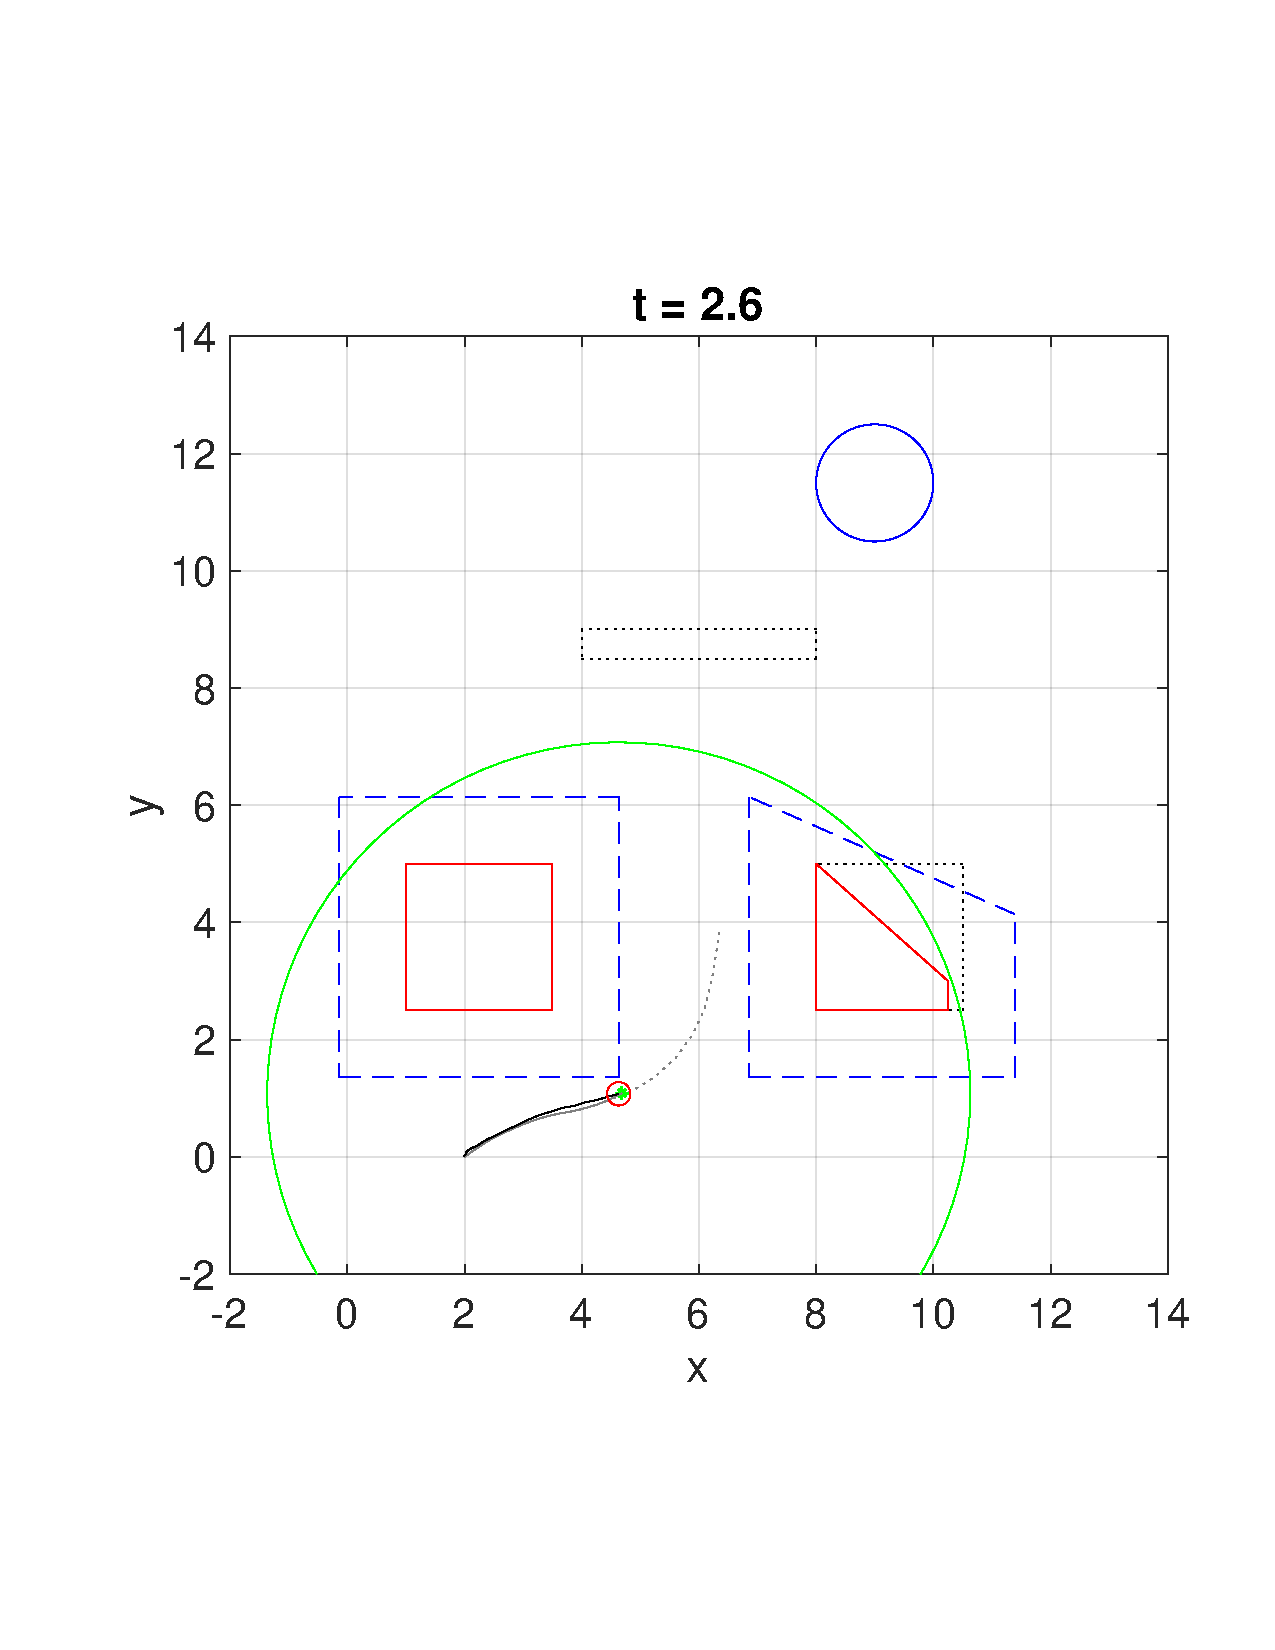
\includegraphics[width=\columnwidth]{fig/Q8D_Q4D/26}
  \end{subfigure}
  \begin{subfigure}[t]{0.49\columnwidth}
    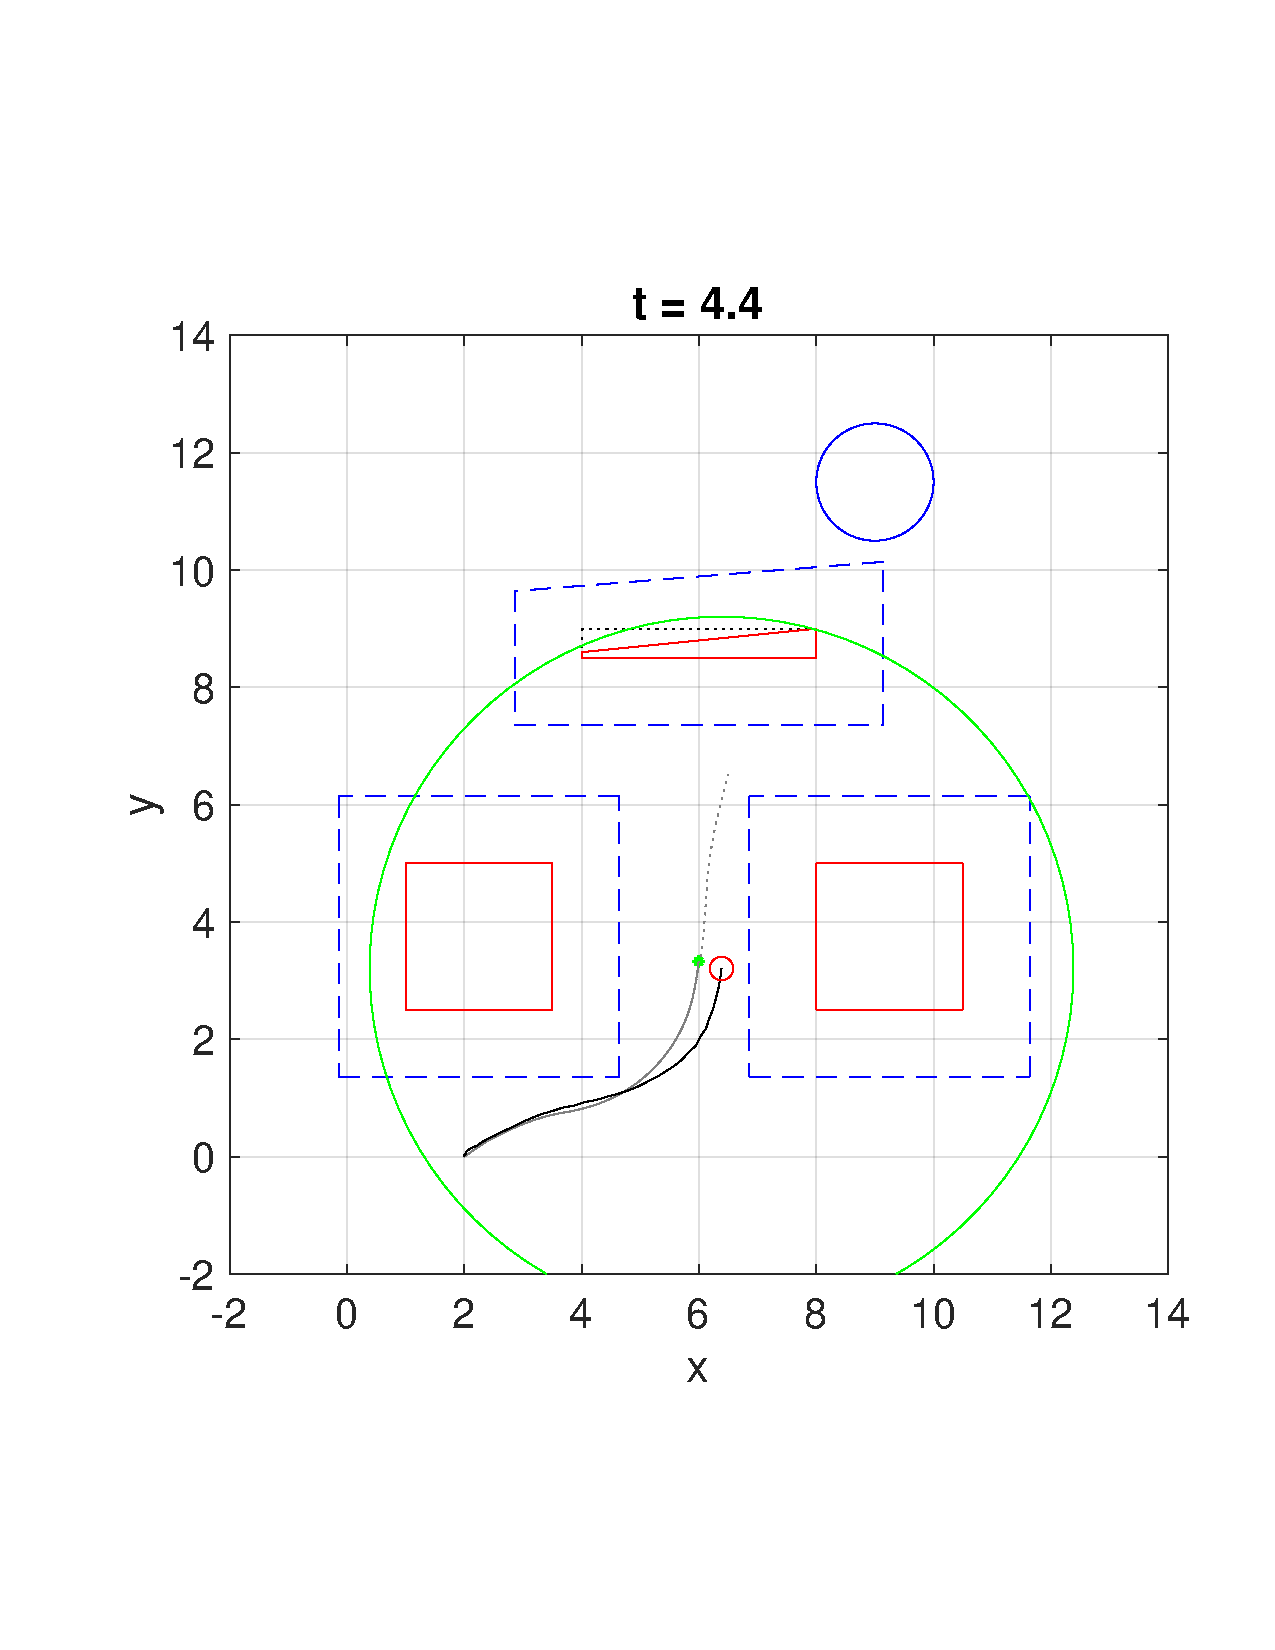
\includegraphics[width=\columnwidth]{fig/Q8D_Q4D/44}
  \end{subfigure}  
  
  \begin{subfigure}[t]{0.49\columnwidth}
    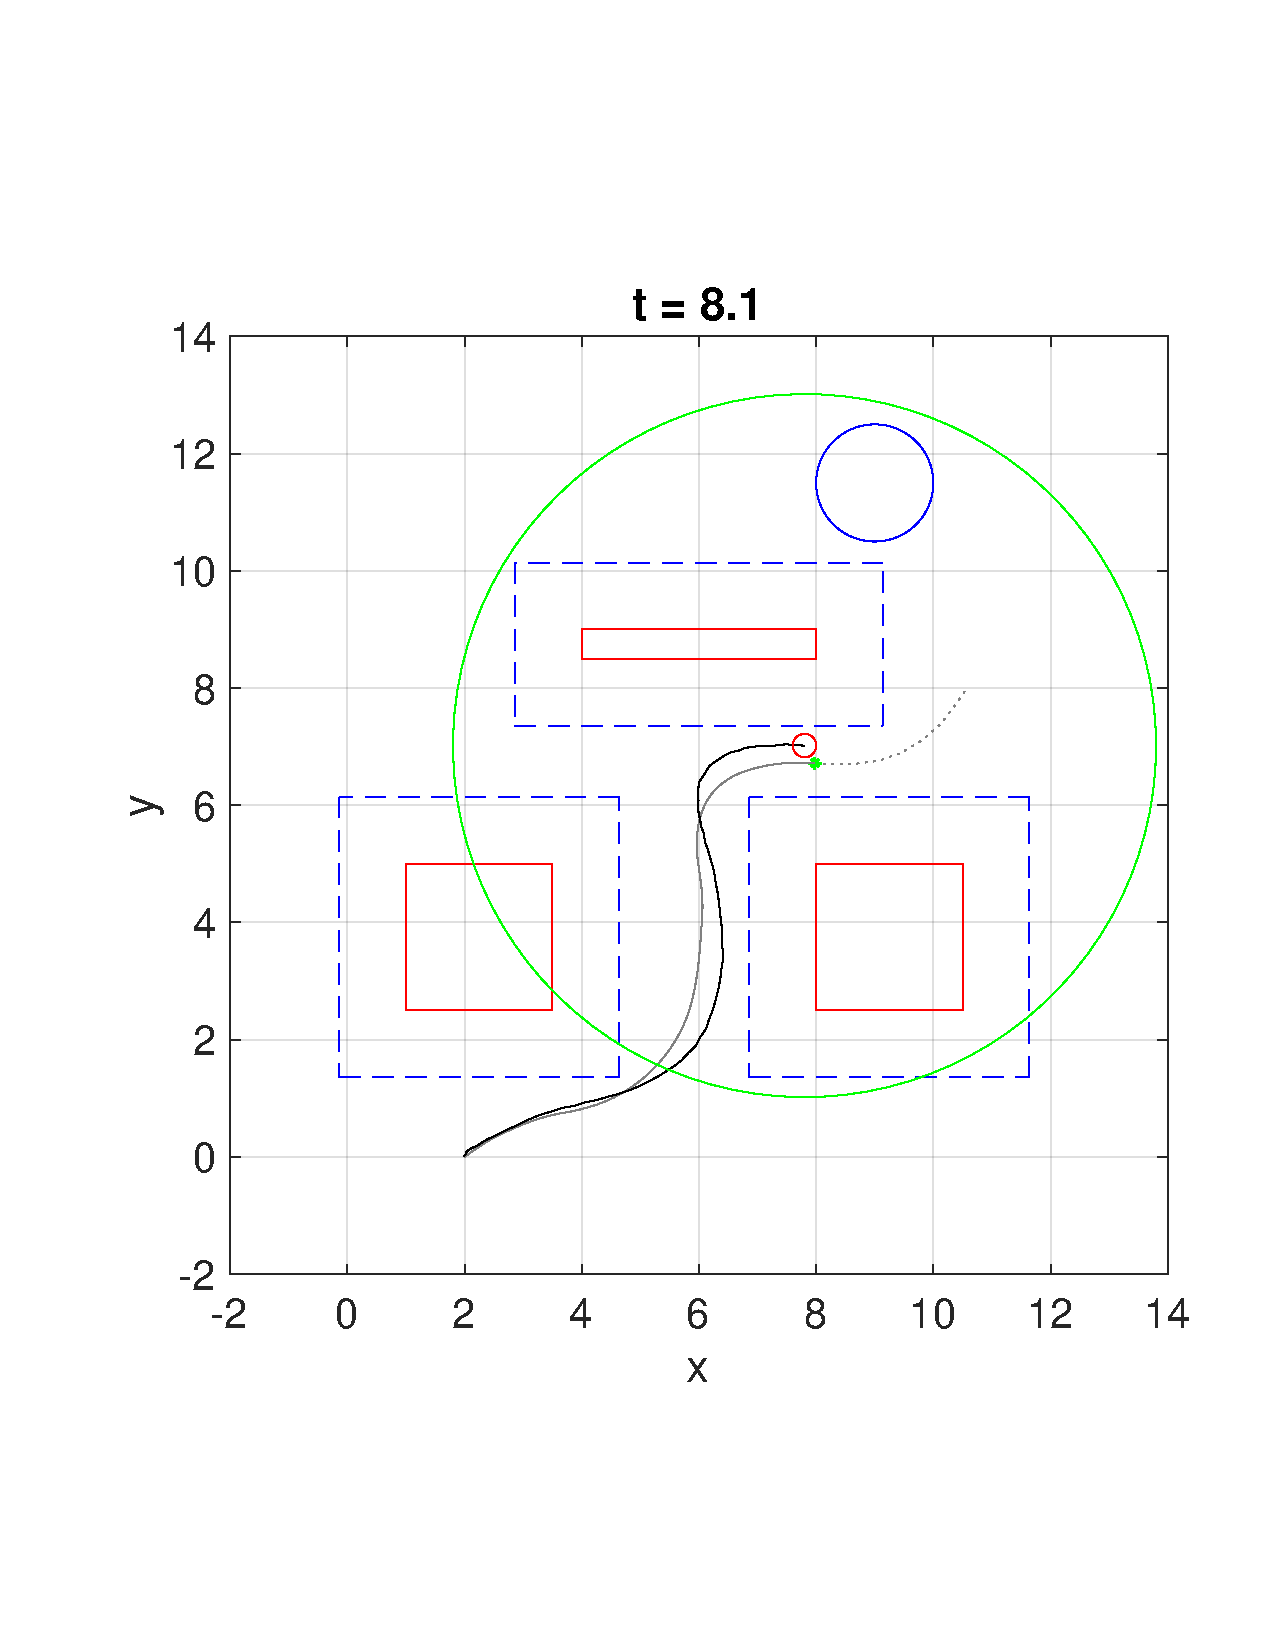
\includegraphics[width=\columnwidth]{fig/Q8D_Q4D/81}
  \end{subfigure}
  \begin{subfigure}[t]{0.49\columnwidth}
    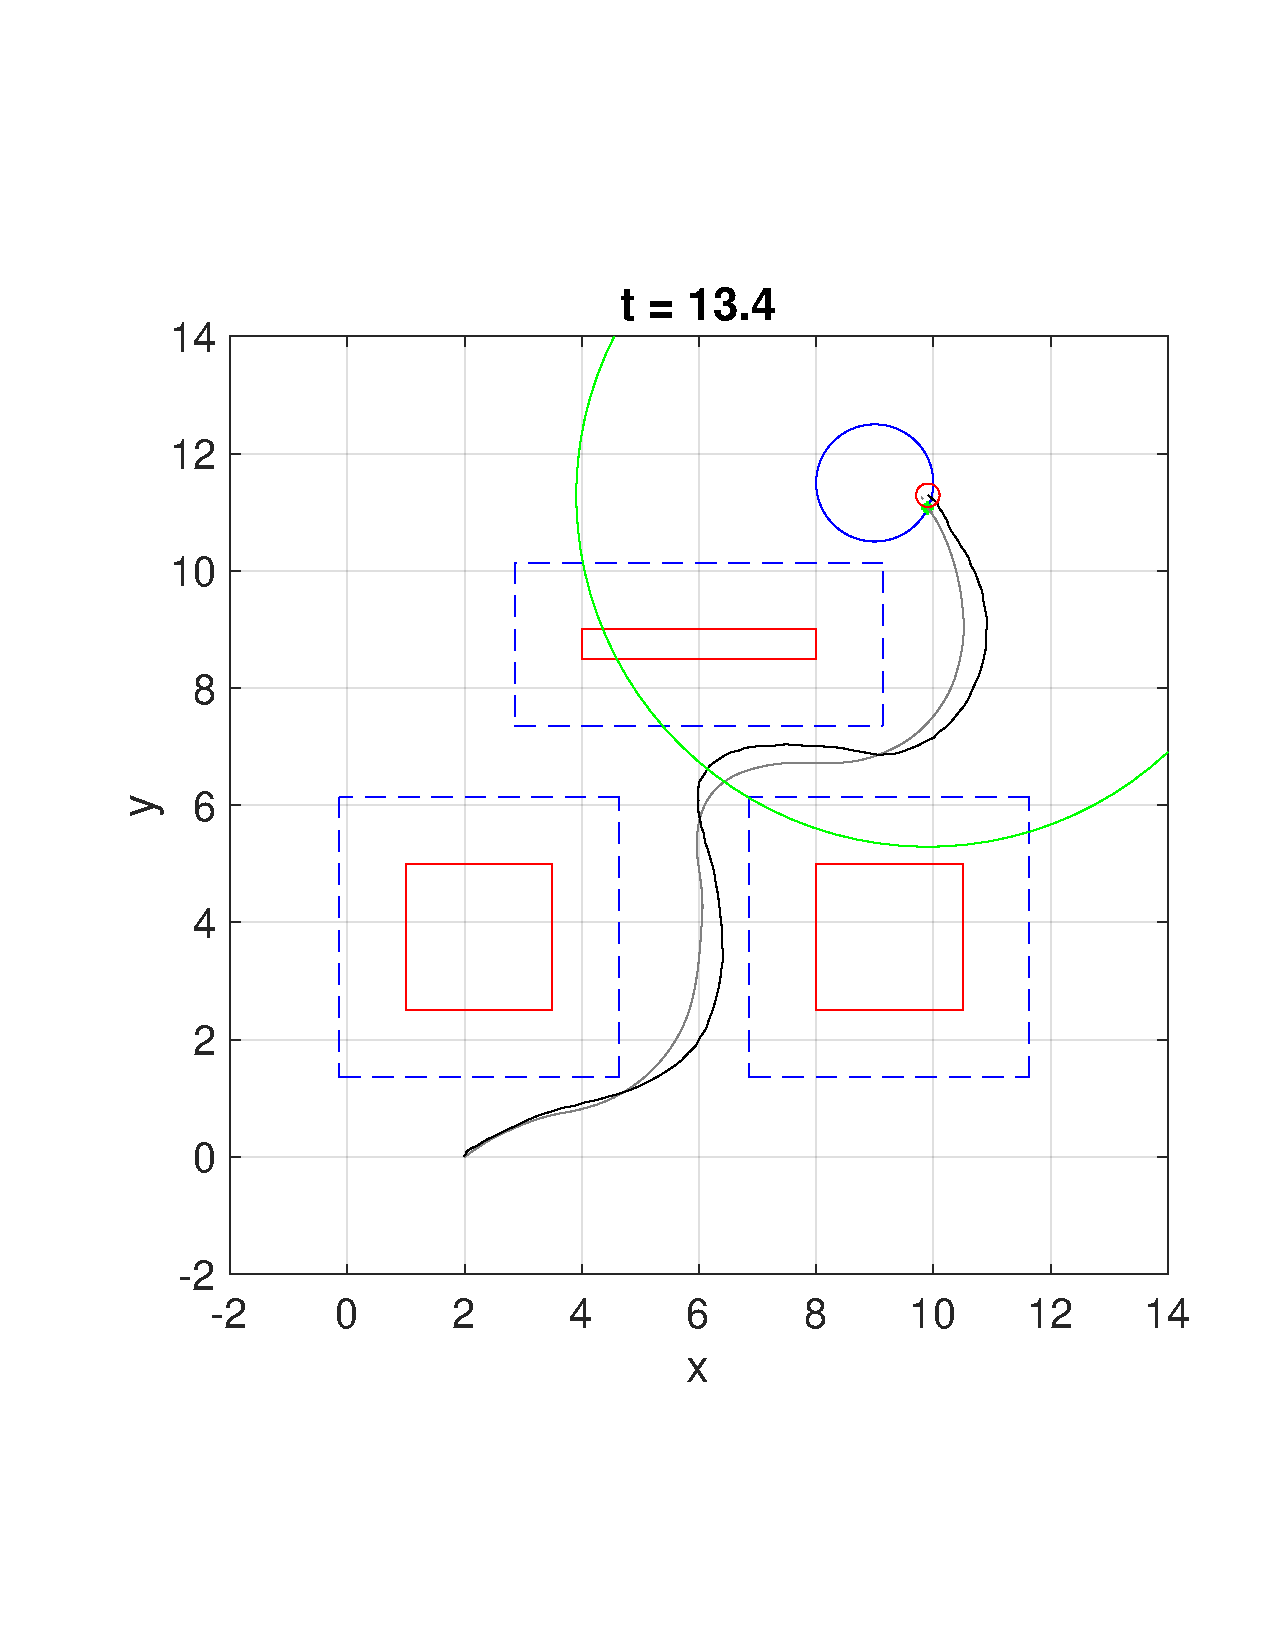
\includegraphics[width=\columnwidth]{fig/Q8D_Q4D/134}
  \end{subfigure}
  \caption{Simulation of the 8D-4D example. As the quadrotor with 8D dynamics (position shown as a red circle) senses new obstacles in the sensing region (light green circle), the 4D model (position shown as a green star) replans trajectories, which are robustly tracked by the 8D system. Augmented obstacles (dashed blue) ensures safety of the 8D system using the optimal tracking controller.} \label{fig:8D4Dsim}
\end{figure}

Fig. \ref{fig:Q8D_tracking_error} shows the tracking error in the positional state $x_r$ over time. The red points indicate the time points at which the optimal tracking controller from Eq. \eqref{eq:opt_ctrl_inf} is used. One can observe that the tracking error is always less than 0.45, well below the minimal TEB of 1.11 implied by the value function in Fig. \ref{fig:vf_TEB:8D4D}.
The disturbance was chosen to be uniformly random within the chosen bounds.

\begin{figure}
  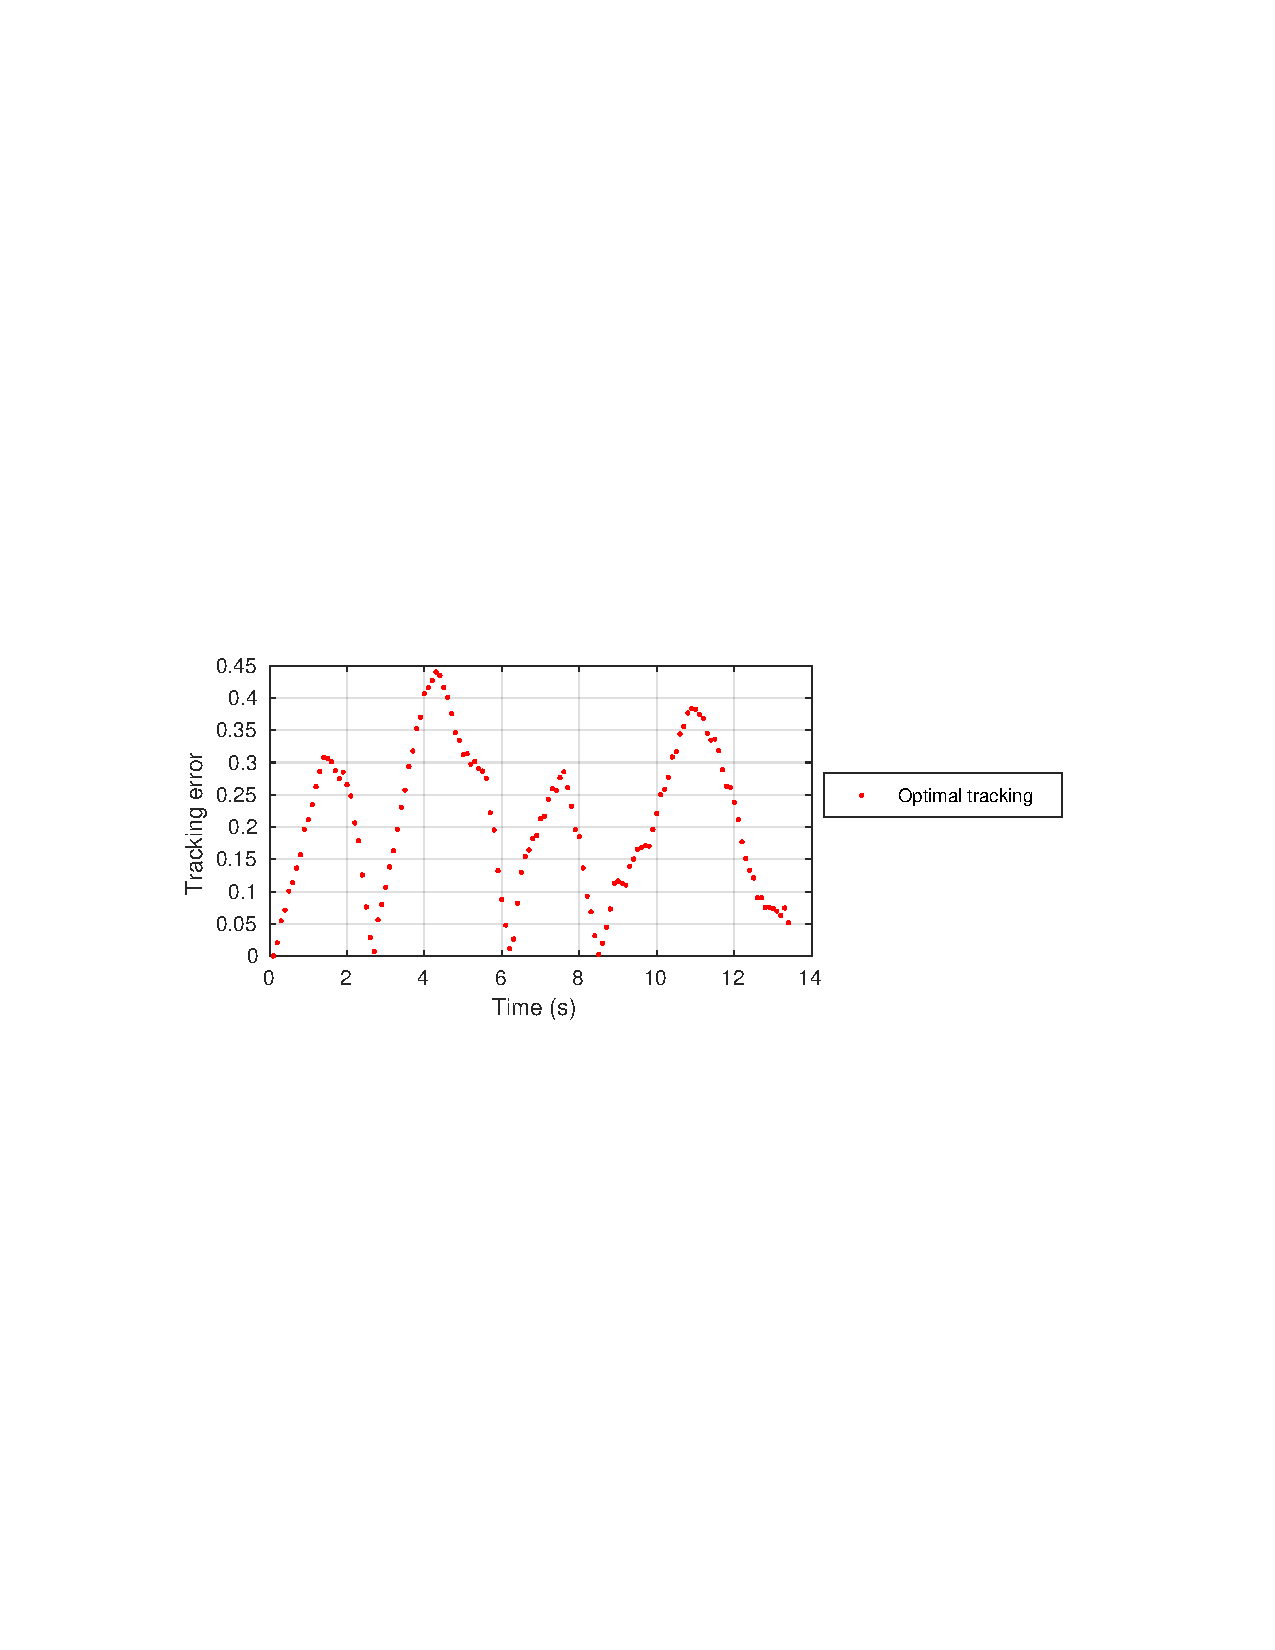
\includegraphics[width=\columnwidth]{fig/Q8D_Q4D/quad8D_tracking_error}
  \caption{Tracking error in $x_{r}$ over time for the 8D-4D example. The error is always well below the minimal TEB of 1.11.}
  \label{fig:Q8D_tracking_error}
\end{figure}

Fig. \ref{fig:Q8D_TVTEB} shows the time-varying TEB in state $v_{x,r}$ used in each MPC planning loop. We compare the simulation time where the time-varying TEB is used for planning with the case in that the TEB is fixed as a constant, and the results are summarized in Table \ref{tab:sim_time}. One can observe that with the use of time-varying TEB the conservatism in planning is reduced and a faster flight time is achieved.

\begin{figure}
  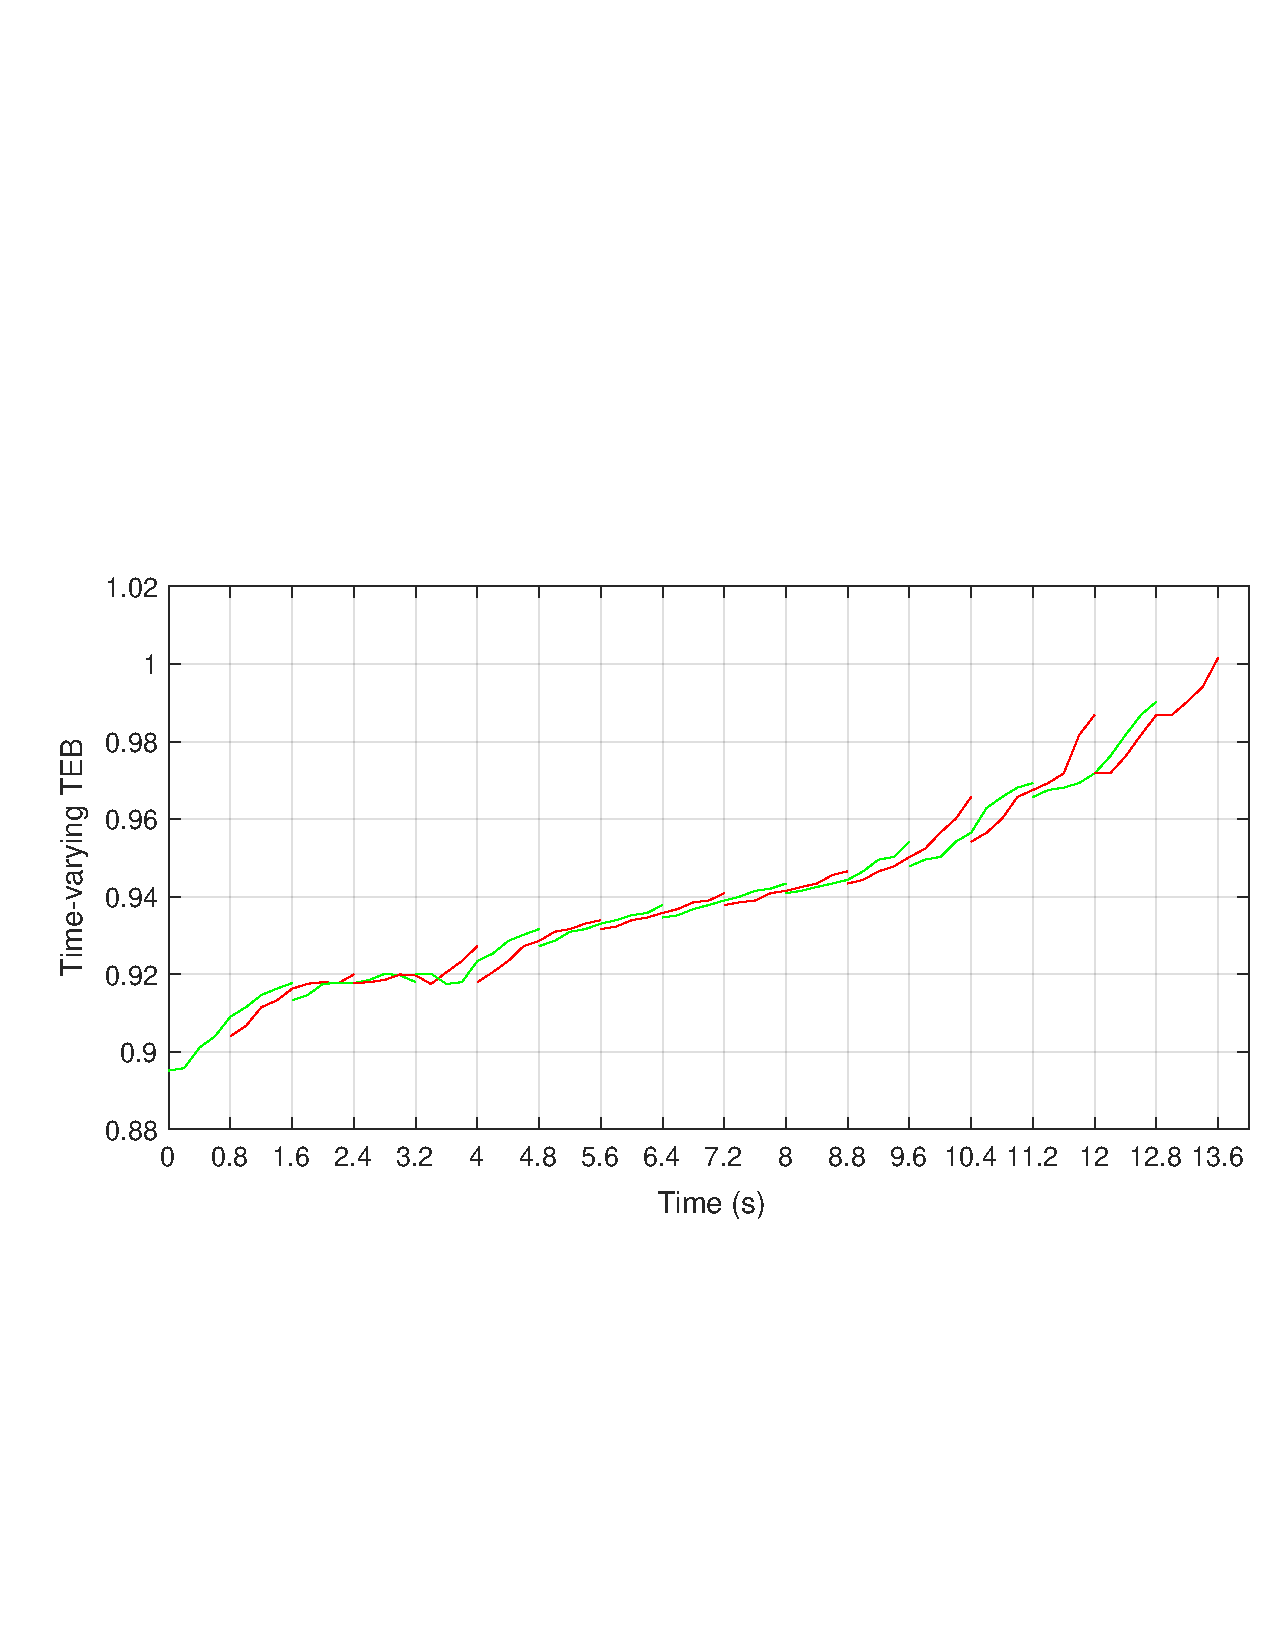
\includegraphics[width=\columnwidth]{fig/Q8D_Q4D/TVTEB}
  \caption{Lists of time-varying tracking error bound in $v_{x,r}$ over time used in MPC planning.}
  \label{fig:Q8D_TVTEB}
\end{figure}

\begin{table}[htbp!]
\caption{\small{Simulation time with constant and time-varying TEB.}}
\centering
\normalsize
\begin{tabular}{ccccc}
\hline
&Simulation case &  Time (s)    \\ 
\hline
&Planning with constant TEB     &  14.6  \\
&Planning with time-varying TEB &  13.4  \\
\hline
\end{tabular}
\label{tab:sim_time}
\end{table}

Implementation of the MPC planner was based on MATLAB and \texttt{ACADO Toolkit} \cite{Houska2011a}. The nonlinear MPC problem was solved using an online active set strategy implemented in \texttt{qpOASES} \cite{Ferreau2014}. All the simulation results were obtained on a laptop with Ubuntu 14.04 LTS operating system and a Core i5-4210U CPU. For the MPC problem we used a horizon $N=8$ with sampling interval $\Delta t_{\text{mpc}} = 0.2$. The planner replans every 0.8 s with an average computational time of 0.37 s for each planning loop. The frequency of control was once every 0.1 s, i.e. $\Delta t = 0.1$ for both the 4D double integrator and 8D quadrotor system.